
\documentclass[aspectratio=169,11pt]{beamer}
\usetheme{default}
\usefonttheme{professionalfonts}
\setbeamertemplate{navigation symbols}{}
\setbeamertemplate{headline}{}
\setbeamertemplate{footline}{%
  \leavevmode\hbox{%
  \begin{beamercolorbox}[wd=.82\paperwidth,ht=2.4ex,dp=1ex,leftskip=1.5em]{author in head/foot}%
  \scriptsize TDOT Slope Movement Monitoring System
  \end{beamercolorbox}%
  \begin{beamercolorbox}[wd=.18\paperwidth,ht=2.4ex,dp=1ex,center]{date in head/foot}%
  \scriptsize \insertframenumber/\inserttotalframenumber
  \end{beamercolorbox}}}
\usepackage[T1]{fontenc}
\usepackage[utf8]{inputenc}
\usepackage{amsmath,amssymb}
\usepackage{booktabs,array,tabularx,ragged2e}
\usepackage{tikz}
\usetikzlibrary{arrows.meta,positioning}
\setbeamercolor{normal text}{fg=black,bg=white}
\setbeamercolor{structure}{fg=black}
\setbeamercolor{frametitle}{fg=black,bg=white}
\setbeamercolor{title}{fg=black,bg=white}
\setbeamercolor{subtitle}{fg=black,bg=white}
\setbeamercolor{author}{fg=black,bg=white}
\setbeamercolor{date}{fg=black,bg=white}
\setbeamercolor{block title}{fg=black,bg=white}
\setbeamercolor{block body}{fg=black,bg=white}
\setbeamercolor{author in head/foot}{fg=black,bg=white}
\setbeamercolor{date in head/foot}{fg=black,bg=white}
\setbeamersize{text margin left=0.65cm,text margin right=0.65cm}
\setbeamerfont{frametitle}{size=\large,series=\bfseries}
\setbeamertemplate{itemize item}{--}
\setbeamertemplate{itemize subitem}{--}
\setlength{\parskip}{1.5pt}
\renewcommand{\arraystretch}{1.16}
\newcommand{\slideheading}[1]{\vspace{0.05cm}\textbf{#1}\vspace{0.12cm}}
\newcolumntype{Y}{>{\RaggedRight\arraybackslash}X}
\newcolumntype{L}[1]{>{\RaggedRight\arraybackslash}p{#1}}
\newcolumntype{C}[1]{>{\centering\arraybackslash}p{#1}}
\begin{document}

\begin{frame}[plain]
\centering
\vspace{0.8cm}
{\Large\bfseries TDOT Slope Movement Monitoring System}\\[0.25cm]
{\normalsize East Tennessee Highway Corridor Risk Assessment}\\[0.8cm]
{\normalsize Momina Ali}\\[0.1cm]
{\small University of Tennessee, Knoxville}\\[0.9cm]
\rule{0.78\textwidth}{0.4pt}\\[0.25cm]
{\small Proof of Concept: I-40 and I-75 Mountain Corridors}\\[0.15cm]
{\small Real Sentinel-1 InSAR, USGS Terrain, USGS Geology, and FHWA Traffic Data}\\[0.25cm]
\rule{0.78\textwidth}{0.4pt}\\[0.55cm]
{\scriptsize GitHub: \texttt{github.com/MominaLAli/tdot-slope-monitoring}}
\end{frame}

\begin{frame}{Problem and Project Objective}
\begin{columns}[T,onlytextwidth]
\begin{column}{0.49\textwidth}
\slideheading{TDOT problem}
\begin{itemize}\setlength\itemsep{0.25em}
  \item Tennessee has many unstable slope sites across highway corridors.
  \item Annual manual inspection of every site is difficult at statewide scale.
  \item Terrain-only screening can miss flat areas that are actively moving.
  \item A decision-support tool is needed to combine movement, terrain, geology, and road exposure.
\end{itemize}
\end{column}
\begin{column}{0.49\textwidth}
\slideheading{Proof-of-concept objective}
\begin{itemize}\setlength\itemsep{0.25em}
  \item Detect real ground movement using Sentinel-1 InSAR.
  \item Extract terrain susceptibility features from USGS 3DEP DEM data.
  \item Integrate geology and traffic exposure into a risk score.
  \item Rank highway segments for inspection priority.
  \item Provide a dashboard that TDOT engineers can use without coding.
\end{itemize}
\end{column}
\end{columns}
\vspace{0.22cm}
\begin{center}
\fbox{\parbox{0.86\textwidth}{\centering\small Key idea: use satellite displacement to identify moving slopes that terrain-only inspection may overlook.}}
\end{center}
\end{frame}

\begin{frame}{Study Area and Data Sources}
\begin{columns}[T,onlytextwidth]
\begin{column}{0.47\textwidth}
\slideheading{Corridors analyzed}
\scriptsize
\begin{tabularx}{\linewidth}{L{1.1cm}Y C{1.15cm} C{1.25cm}}
\toprule
\textbf{Road} & \textbf{Section} & \textbf{Length} & \textbf{Segments} \\
\midrule
I-40 & Cookeville to North Carolina border & 274 km & 342 \\
I-75 & Jellico Mountain section, Campbell County & 72 km & 90 \\
\midrule
\textbf{Total} & East Tennessee & \textbf{346 km} & \textbf{432} \\
\bottomrule
\end{tabularx}
\end{column}
\begin{column}{0.50\textwidth}
\slideheading{Input layers}
\scriptsize
\begin{tabularx}{\linewidth}{L{2.25cm}Y}
\toprule
\textbf{Layer} & \textbf{Source and role} \\
\midrule
InSAR & Sentinel-1 via ASF HyP3; 35 pairs from Jan. 2022-Jan. 2024 \\
Terrain & USGS 3DEP 30 m DEM; slope, roughness, curvature, relief \\
Geology & USGS Tennessee geology map; rock type per segment \\
Traffic & FHWA HPMS 2022; AADT and truck percentage \\
\bottomrule
\end{tabularx}
\end{column}
\end{columns}
\vspace{0.25cm}
{\footnotesize All layers are real and publicly available. The analysis uses 0.5-mile segment units and a 500 m buffer for spatial feature extraction.}
\end{frame}

\begin{frame}{Processing Pipeline}
\centering
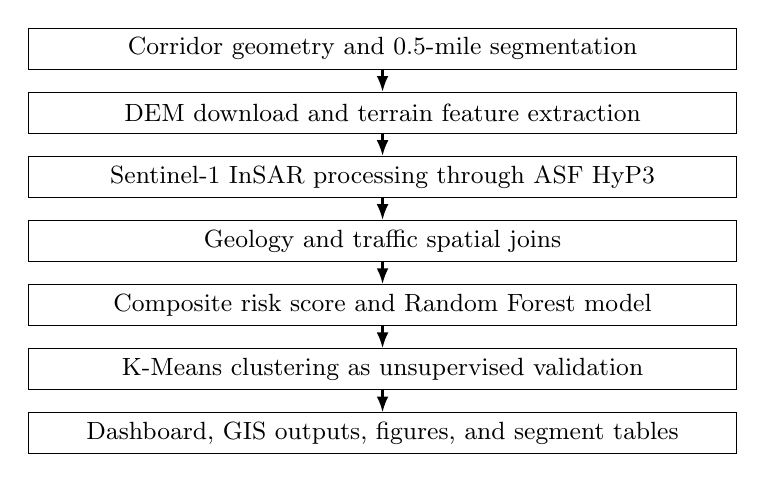
\begin{tikzpicture}[node distance=0.28cm,box/.style={rectangle,draw,minimum width=9.0cm,minimum height=0.52cm,align=center,font=\small},arrow/.style={-{Latex[length=2mm]},thick}]
\node[box] (a) {Corridor geometry and 0.5-mile segmentation};
\node[box,below=of a] (b) {DEM download and terrain feature extraction};
\node[box,below=of b] (c) {Sentinel-1 InSAR processing through ASF HyP3};
\node[box,below=of c] (d) {Geology and traffic spatial joins};
\node[box,below=of d] (e) {Composite risk score and Random Forest model};
\node[box,below=of e] (f) {K-Means clustering as unsupervised validation};
\node[box,below=of f] (g) {Dashboard, GIS outputs, figures, and segment tables};
\draw[arrow] (a)--(b); \draw[arrow] (b)--(c); \draw[arrow] (c)--(d); \draw[arrow] (d)--(e); \draw[arrow] (e)--(f); \draw[arrow] (f)--(g);
\end{tikzpicture}\par
\vspace{0.22cm}
{\footnotesize The pipeline converts raw geospatial and satellite products into ranked segment-level inspection priorities.}
\end{frame}

\begin{frame}{Risk Score Formulation}
\slideheading{Composite risk score}
\small
\begin{equation*}
\begin{aligned}
\text{Risk} ={}& 0.35P_{ML} + 0.25S_{terrain} + 0.20S_{InSAR} \\
&+ 0.12S_{road} + 0.08S_{geo}
\end{aligned}
\end{equation*}
\vspace{0.15cm}
\scriptsize
\begin{tabularx}{0.92\linewidth}{L{2.6cm}Y}
\toprule
\textbf{Component} & \textbf{Meaning} \\
\midrule
$P_{ML}$ & Random Forest probability of slope-risk class \\
$S_{terrain}$ & Mean slope, elevation range, and terrain roughness \\
$S_{InSAR}$ & Mean displacement, displacement trend, and displacement variability \\
$S_{road}$ & AADT and truck volume exposure \\
$S_{geo}$ & Rock-type susceptibility score \\
\bottomrule
\end{tabularx}
\vspace{0.25cm}

{\footnotesize All continuous variables are min-max normalized before the weighted score is calculated.}
\end{frame}

\begin{frame}{Risk Category Results}
\centering
\small
\begin{tabular}{lcccc}
\toprule
\textbf{Risk Category} & \textbf{Score Range} & \textbf{I-40} & \textbf{I-75} & \textbf{Total} \\
\midrule
Low & 0.00-0.25 & 242 & 53 & 295 \\
Moderate & 0.25-0.50 & 34 & 10 & 44 \\
High & 0.50-0.75 & 66 & 25 & 91 \\
Critical & 0.75-1.00 & 0 & 2 & 2 \\
\midrule
\textbf{Total} & & \textbf{342} & \textbf{90} & \textbf{432} \\
\bottomrule
\end{tabular}
\vspace{0.45cm}
\begin{itemize}\setlength\itemsep{0.3em}
  \item Most segments are Low risk, but 93 segments are High or Critical.
  \item The two Critical segments are both located on the I-75 Jellico section.
  \item The category thresholds provide an inspection-priority ranking rather than a final engineering diagnosis.
\end{itemize}
\end{frame}

\begin{frame}{Machine Learning Model Performance}
\begin{columns}[T,onlytextwidth]
\begin{column}{0.52\textwidth}
\slideheading{Model comparison}
\scriptsize
\begin{tabularx}{\linewidth}{Y C{2.6cm}}
\toprule
\textbf{Model} & \textbf{5-fold CV ROC-AUC} \\
\midrule
Random Forest, I-40 only & $0.952 \pm 0.055$ \\
Random Forest, combined corridors & $0.945 \pm 0.050$ \\
Gradient Boosting & $0.986 \pm 0.006$ \\
Logistic Regression & $0.997 \pm 0.002$ \\
\bottomrule
\end{tabularx}
\end{column}
\begin{column}{0.43\textwidth}
\slideheading{Interpretation note}
\footnotesize
High AUC values reflect proxy labels derived from the same feature space. These results are useful for proof-of-concept testing, but they should be recalibrated after TDOT USMP inspection points are available.
\vspace{0.3cm}

\slideheading{Primary model}
\footnotesize
Random Forest was selected as the main model because it handles mixed data types, nonlinear relationships, and feature-importance estimation.
\end{column}
\end{columns}
\end{frame}


\begin{frame}{Unsupervised Validation}
\begin{columns}[T,onlytextwidth]
\begin{column}{0.48\textwidth}
\slideheading{K-Means cluster profiles}
\scriptsize
\begin{tabular}{cccc}
\toprule
\textbf{Cluster} & \textbf{Risk} & \textbf{N} & \textbf{Mean slope} \\
\midrule
0 & Moderate & 149 & 5.2$^\circ$ \\
1 & Low & 128 & 4.1$^\circ$ \\
2 & High & 65 & 13.7$^\circ$ \\
\bottomrule
\end{tabular}
\vspace{0.25cm}
\begin{itemize}\setlength\itemsep{0.25em}\footnotesize
  \item Cluster 0: displacement-driven moderate risk
  \item Cluster 1: flat-terrain low risk
  \item Cluster 2: steep-terrain high risk
\end{itemize}
\end{column}
\begin{column}{0.48\textwidth}
\slideheading{Why this is important}
\footnotesize
K-Means was applied directly to real feature measurements with no proxy labels. The clustering results are consistent with the supervised model, suggesting that the terrain and InSAR signals are meaningful before USMP ground-truth validation.
\vspace{0.25cm}
\begin{itemize}\setlength\itemsep{0.25em}
  \item Optimal K: 3
  \item Silhouette score: 0.376
  \item PCA variance explained: 67.2\% in first two components
\end{itemize}
\end{column}
\end{columns}
\end{frame}

\begin{frame}{Key Finding: Segment 149 on I-40}
\begin{columns}[T,onlytextwidth]
\begin{column}{0.48\textwidth}
\slideheading{Segment profile}
\scriptsize
\begin{tabularx}{\linewidth}{L{2.45cm}Y}
\toprule
\textbf{Property} & \textbf{Value} \\
\midrule
Location & I-40, east of Knoxville \\
Mean slope & 5.2$^\circ$ \\
Rock class & Carbonate limestone \\
Valid InSAR pairs & 32 of 35 \\
Mean displacement & -3.318 mm \\
Trend & \textbf{-1.785 mm/month} \\
Cumulative movement & Approx. -43 mm over two years \\
Mean coherence & 0.420 \\
\bottomrule
\end{tabularx}
\end{column}
\begin{column}{0.48\textwidth}
\slideheading{Why this matters}
\small
\begin{itemize}\setlength\itemsep{0.35em}
  \item The segment is relatively flat, so terrain-only screening classifies it as low risk.
  \item Real Sentinel-1 InSAR indicates sustained subsidence over two years.
  \item The integrated model elevates the segment to high risk.
\end{itemize}
\vspace{0.2cm}
\fbox{\parbox{0.92\linewidth}{\small Segment 149 demonstrates the central value of InSAR: it can identify movement that terrain-only inspection would likely miss.}}
\end{column}
\end{columns}
\end{frame}

\begin{frame}{Additional Findings}
\begin{columns}[T,onlytextwidth]
\begin{column}{0.48\textwidth}
\slideheading{I-75 Jellico critical segments}
\begin{itemize}\setlength\itemsep{0.3em}\small
  \item Segments 1023 and 1024 in Campbell County are classified as Critical.
  \item Risk scores are 0.797 and 0.800.
  \item Both segments have clastic sedimentary rock and slopes near 15.5$^\circ$.
  \item Findings are consistent with known Jellico-area slope concerns.
\end{itemize}
\end{column}
\begin{column}{0.48\textwidth}
\slideheading{Geology and risk}
\scriptsize
\begin{tabularx}{\linewidth}{Y C{1.0cm} C{1.8cm}}
\toprule
\textbf{Rock class} & \textbf{N} & \textbf{High/Critical} \\
\midrule
Metamorphic/crystalline & 1 & 1 \\
Clastic sedimentary & 186 & 91 \\
Other & 70 & 2 \\
Carbonate & 175 & 0 \\
\bottomrule
\end{tabularx}
\vspace{0.2cm}
{\footnotesize Clastic sedimentary units account for 91 of 93 High/Critical segments, making geology a major risk discriminator in the current study area.}
\end{column}
\end{columns}
\end{frame}


\begin{frame}{Dashboard}
\slideheading{Six dashboard tabs}
\footnotesize
\begin{columns}[T,onlytextwidth]
\begin{column}{0.48\textwidth}
\begin{itemize}\setlength\itemsep{0.35em}
  \item \textbf{Risk Map}: interactive segment risk map
  \item \textbf{Analysis}: risk profiles and feature importance
  \item \textbf{Geology and InSAR}: rock type, coherence, displacement
\end{itemize}
\end{column}
\begin{column}{0.48\textwidth}
\begin{itemize}\setlength\itemsep{0.35em}
  \item \textbf{Corridor Compare}: I-40 versus I-75 metrics
  \item \textbf{Segment Table}: filterable table and CSV export
  \item \textbf{Risk Clustering}: K-Means PCA and Segment 149 analysis
\end{itemize}
\end{column}
\end{columns}
\vspace{0.45cm}
\begin{center}
\fbox{\parbox{0.70\textwidth}{\centering\footnotesize Run command: \texttt{streamlit run streamlit\_app.py}}}
\end{center}
\end{frame}


\begin{frame}{Deliverables}
\slideheading{Main project outputs}
\footnotesize
\begin{columns}[T,onlytextwidth]
\begin{column}{0.48\textwidth}
\begin{itemize}\setlength\itemsep{0.35em}
  \item GIS-ready risk segment GeoJSON
  \item Standalone interactive HTML map
  \item Top-risk segment table for inspection priority
\end{itemize}
\end{column}
\begin{column}{0.48\textwidth}
\begin{itemize}\setlength\itemsep{0.35em}
  \item Feature-importance table for model interpretation
  \item Unsupervised clustering figure
  \item Segment 149 deep-dive figure
\end{itemize}
\end{column}
\end{columns}
\vspace{0.45cm}
\begin{center}
\fbox{\parbox{0.82\textwidth}{\centering\footnotesize These outputs support engineering review and inspection prioritization. They do not replace field inspection or geotechnical judgment.}}
\end{center}
\end{frame}

\begin{frame}{Limitations and Next Steps}
\begin{columns}[T,onlytextwidth]
\begin{column}{0.48\textwidth}
\slideheading{Current limitations}
\begin{itemize}\setlength\itemsep{0.3em}\small
  \item Proxy labels are not a substitute for TDOT USMP ground truth.
  \item I-75 InSAR processing is pending.
  \item Standard k-fold cross-validation may overestimate performance for spatial data.
  \item 30 m DEM data may miss fine-scale slope features.
\end{itemize}
\end{column}
\begin{column}{0.48\textwidth}
\slideheading{Recommended next steps}
\begin{enumerate}\setlength\itemsep{0.3em}\small
  \item Obtain TDOT USMP inspection points for validation.
  \item Submit I-75 ASF HyP3 InSAR jobs.
  \item Implement spatial block cross-validation.
  \item Add higher-resolution Tennessee LiDAR data.
  \item Extend to I-81, US-441, and US-64.
\end{enumerate}
\end{column}
\end{columns}
\end{frame}

\begin{frame}{Conclusion}
\begin{itemize}\setlength\itemsep{0.45em}
  \item The project demonstrates an end-to-end slope monitoring workflow for TDOT using real public datasets.
  \item The system covers 432 highway segments across 346 km of East Tennessee corridors.
  \item Segment 149 shows that InSAR can detect sustained movement on terrain that would otherwise appear low risk.
  \item I-75 Jellico results show that the method also identifies steep, geologically susceptible critical segments.
  \item The most important next step is ground-truth validation with TDOT USMP data.
\end{itemize}
\vspace{0.35cm}
\begin{center}
\fbox{\parbox{0.82\textwidth}{\centering\small InSAR-integrated monitoring can help prioritize inspection by detecting both visible terrain risk and hidden ground movement.}}
\end{center}
\end{frame}

\end{document}
